\documentclass{tufte-handout}

\usepackage[utf8]{inputenc}
\usepackage[T1]{fontenc}
\usepackage[french]{babel}
\usepackage{indentfirst}

\usepackage{hyperref}

\usepackage{graphicx}

\usepackage{amsmath}
\usepackage{upgreek}
\usepackage{bm}

\usepackage{siunitx}

\usepackage{listings}
\usepackage{xcolor}
\lstset { %
    language=C++,
    backgroundcolor=\color{black!5}, % set backgroundcolor
    basicstyle=\footnotesize,% basic font setting
}

\newcommand\tab[1][1cm]{\hspace*{#1}}

\renewcommand\vec[1]{\bm{\mathrm{#1}}}
\newcommand\unitvec[1]{\bm{\hat{\mathrm{#1}}}}

\title{Dynamique moléculaire de disques durs}
\author{Samuel Diebolt}

\begin{document}

  \maketitle

  \begin{marginfigure}%
    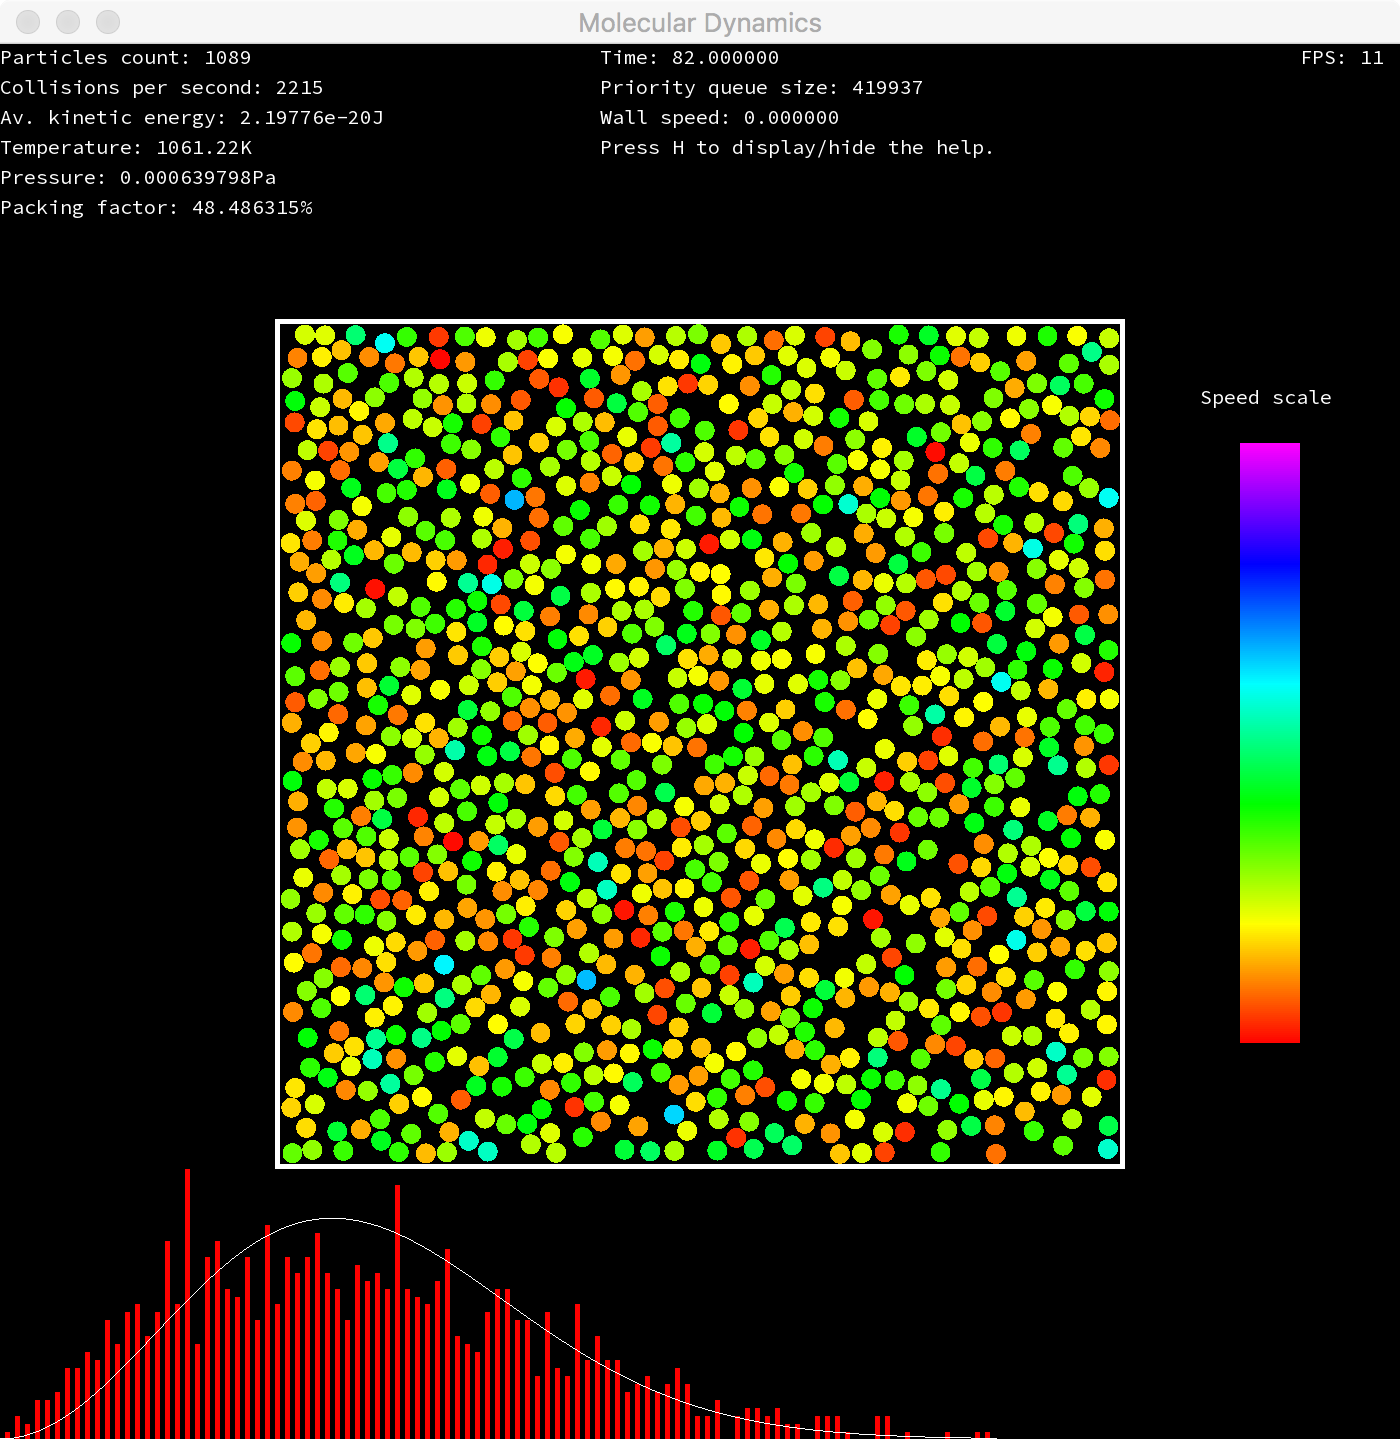
\includegraphics[width=\linewidth]{figures/cover.png}
  \end{marginfigure}

  \begin{abstract}
    Le but de cet exercice est de réaliser une simulation de dynamique moléculaire : on considère un ensemble de particules à l'intérieur d'une boîte à deux dimensions où l'énergie cinétique est conservée. Ces particules répondent donc aux lois des chocs élastiques.
  \end{abstract}

  \section{Description succinte du programme}
  Ci-dessous sont décrites les classes, fonctions et variables les plus importantes du programme, afin d'en comprendre le fonctionnement général. L'intégralité du code est par ailleurs commenté afin d'en faciliter la lecture.
  \begin{itemize}
    \item \textbf{class CollisionSystem} : cette classe est la description du système de simulation.
    \begin{itemize}
      \item \textbf{CollisionSystem$::$Simulate} : fonction de simulation principale, comprenant la boucle de simulation, la gestion des évènements, l'appel aux fonctions d'affichage, etc.

      \item \textbf{std$::$priority\_queue pq\_} : file de priorité permettant de trier les évènements (collisions particule-particule, affichage, etc.).

      \item \textbf{CollisionSystem$::$Predict} : fonction de prédiction des évènements futurs -- collisions entre particules et particule-paroi -- pour une particule considérée.
    \end{itemize}

    \item \textbf{class Particle} : cette classe est la description d'une particule : caractéristiques physiques, éléments graphiques, etc.
    \begin{itemize}
      \item \textbf{Particle$::$TimeToHit$\dots$} : ces fontions renvoient le temps devant s'écouler avant une colision entre la particule considérée et une autre particule ou une des parois.
    \end{itemize}

    \item \textbf{class Event} : cette classe est la description d'un évènement : collisions entre particules, entre particules et parois et affichage de l'état du système sur l'interface graphique.
    \begin{itemize}
      \item \textbf{Event$::$IsValid} : afin d'optimiser les performances\footnote{L'usage mémoire est toutefois considérable lorsque le nombre de collisions par seconde devient trop grand ou lorsque la simulation est laissée en fonctionement pendant un long moment !}, chaque évènement est traité comme suit :
      \begin{enumerate}
        \item Le prochain évènement dans la file de priorité dont les particules considérées n'ont pas subi de collisions entre cet instant et l'ajout antérieur de l'évènement est considéré comme valide et va être traité.

        \item L'état du système est avancé jusqu'au temps de l'évènement.

        \item L'évènement est résolu et l'état du système est mis à jour en conséquence : collision, affichage, etc.

        \item Les futurs évènements concernant la ou les particules considérées sont calculés et ajoutés à la file de priorité.
      \end{enumerate}

      Ainsi, la file de priorité n'est jamais vidée et il n'est nécessaire de calculer que deux prédictions par tour de boucle : on passe d'une complexité de $O(N^2)$ à $O(N)$\footnote{Cette complexité serait encore plus faible en utilisant un arbre pour le traitement des évènements plutôt qu'une file de priorité, ce qui permettrait notamment une suppression des évènements moins coûteuse.}.
    \end{itemize}
  \end{itemize}

  \section{Implémentations}
  La simulation actuelle comporte les éléments suivants :
  \begin{itemize}
    \item Dimensionnement réalisé par les macros du fichier main.h.

    \item Possibilité de rendre le système non-élastique en ajoutant de la friction dans les chocs entre particules.

    \item Affichage des caractéristiques physiques de la simulation : température, pression, compacité.

    \item Affichage des sphères d'influence\footnote{Cette effet purement esthétique est basé sur la technique des metaballs (\url{https://fr.wikipedia.org/wiki/Metaballs}). Il est très coûteux en calculs et doit s'utiliser avec un nombre très limité de particules (5 tout au plus) pour que l'effet soit observé.}.

    \item Affichage de l'histogramme des vitesses – normalisé par rapport à la vitesse la plus représentée – et de la fonction de densité de probabilité de Maxwell-Boltzmann.

    \item Changement de la taille de la boîte de simulation à l'aide des touches directionnelles\footnote{Cela cause des recouvrement de particules en l'état, du fait d'une mauvaise gestion des collisions sur les parois en mouvement.}.

    \item Possiblité d'ajout d'une nouvelle particule de rayon moitié et de masse un quart à une position aléatoire.

    \item Affichage du chemin d'une particule -- mouvement brownien\footnote{Retirer l'affichage des particules à l'aide de la touche P rend l'observation du chemin plus aisée.}.
  \end{itemize}

  \section{Observations et comportements}
  \subsection{Loi de Maxwell-Boltzmann}
  On observe à partir de quelques centaines de particules que la forme de l'histogramme des vitesses est similaire à la fonction de densité de probabilité de Maxwell-Boltzmann et ce très rapidement après le lancement de la simulation, alors que les vitesses sont d'abord générée aléatoirement à l'aide d'une loi uniforme.

  \subsection{Détente adiabatique}
  Sans friction, en réalisant une compression lente puis une détente rapide sur un nombre conséquent de particules (quelques centaines), on observe la figure typique d'une détente adiabatique, les vitesses des particules les plus éloignées étant les plus hautes.
  \begin{marginfigure}
    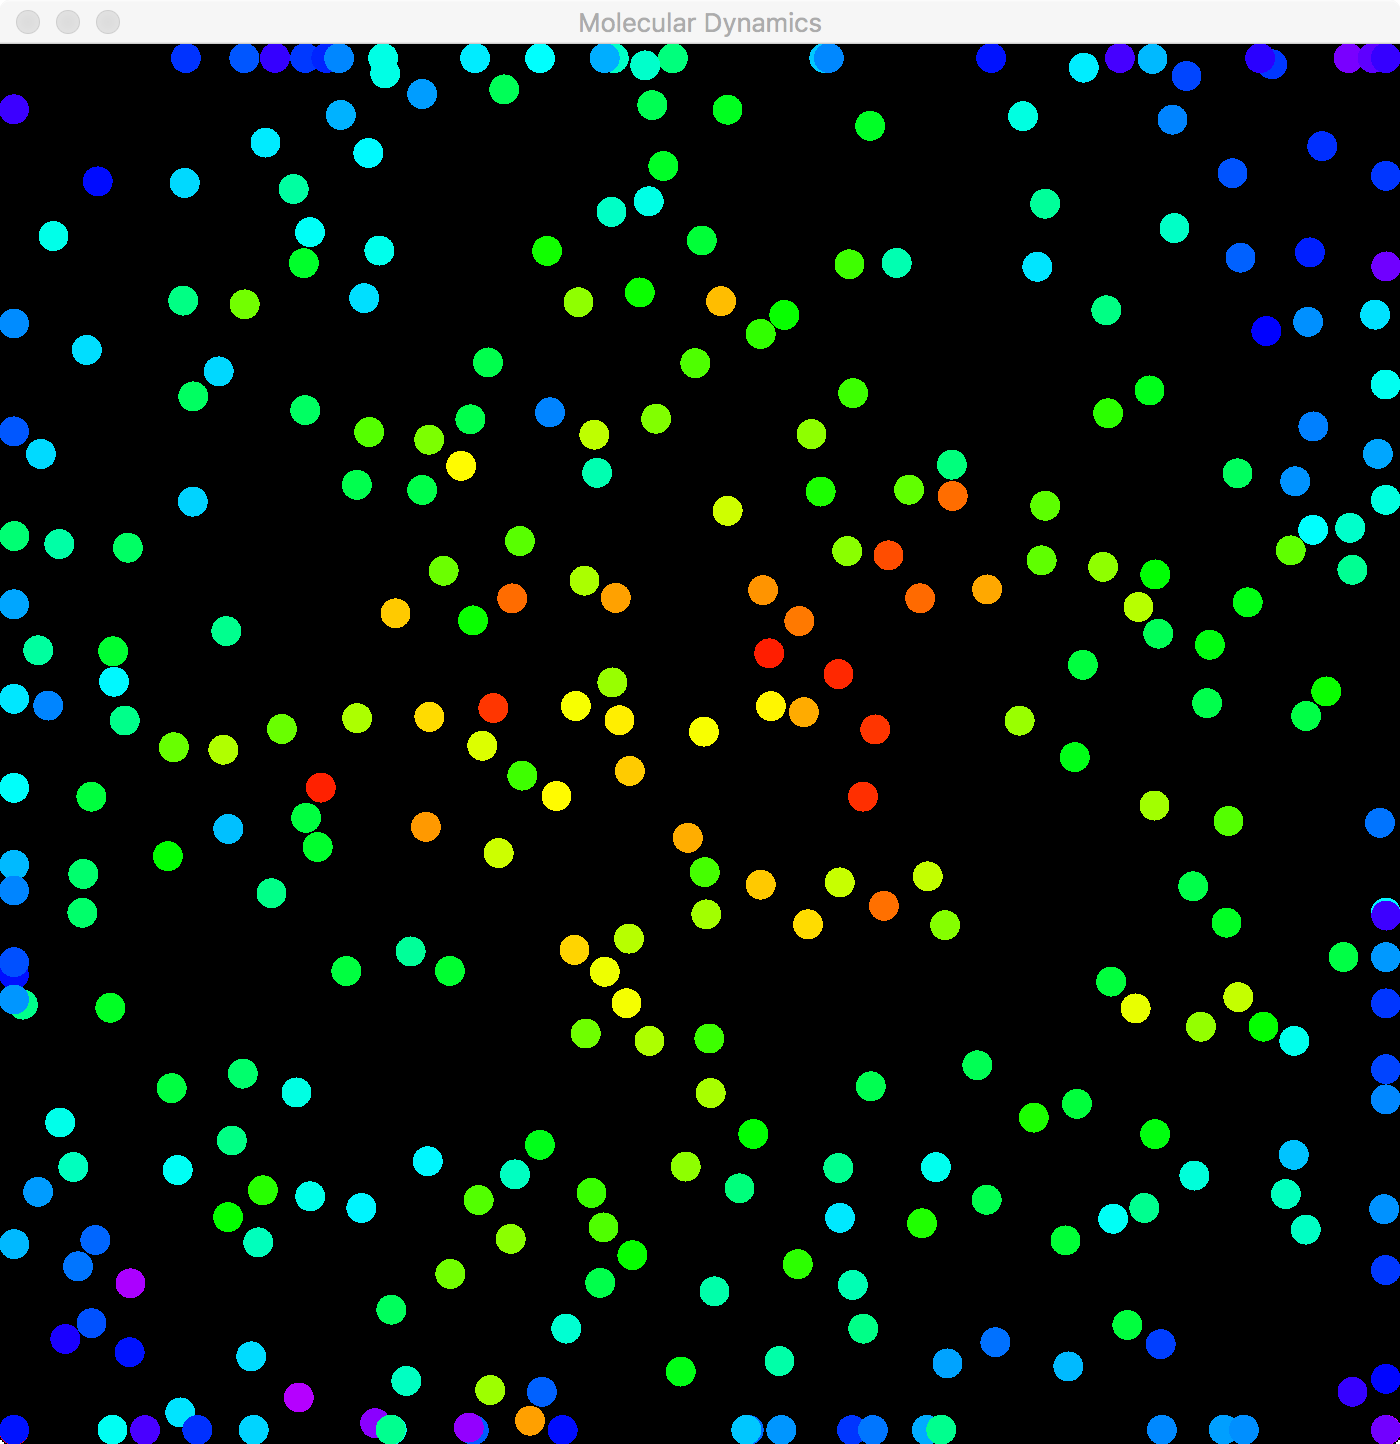
\includegraphics[width=\linewidth]{figures/adiabaticwithoutfriction.png}
    \caption{Détente adiabatique avec les paramètres 15 15 1}
  \end{marginfigure}

  Avec friction en revanche, on observe une figure différente, la détente étant dirigée de façon symétrique selon les faces de la boîte. Cela n'est toutefois pas étonnant, du fait que les particules collées aux parois subissent moins les frictions et sont accélérées par le mouvement des parois.
  \begin{marginfigure}
    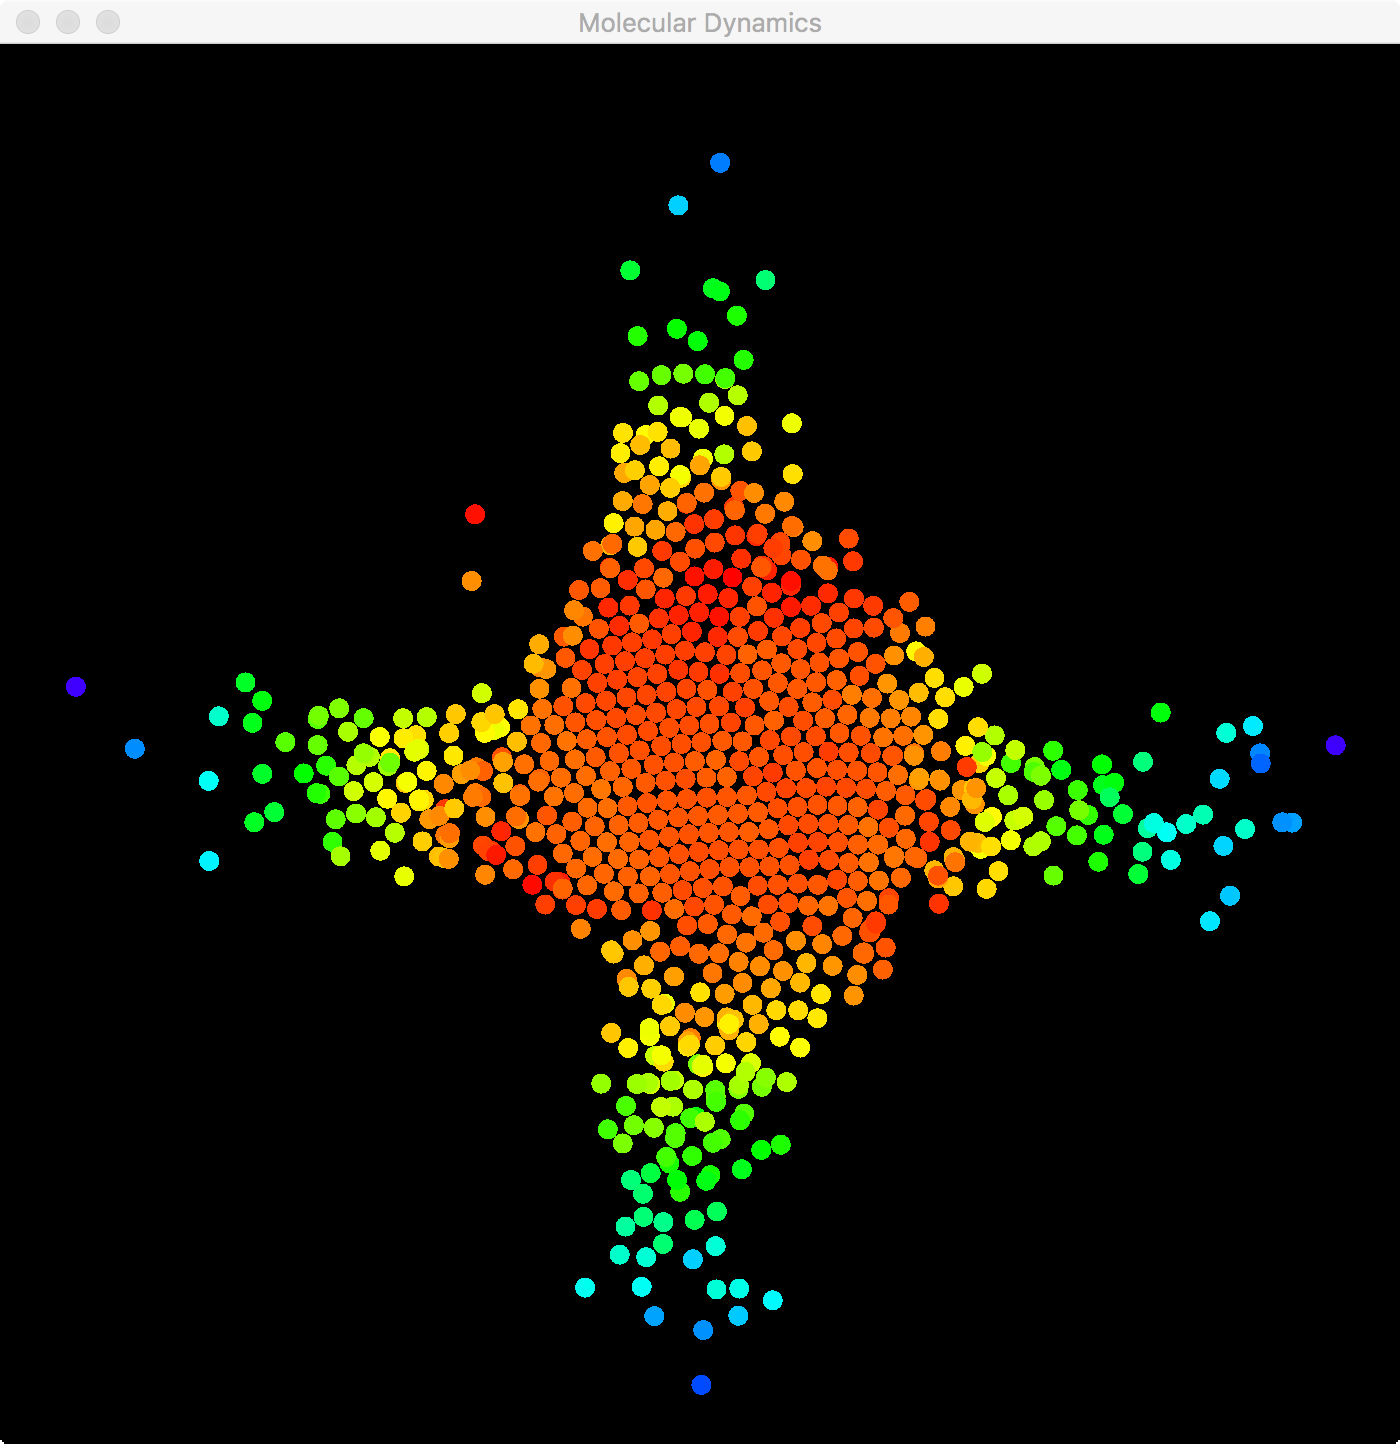
\includegraphics[width=\linewidth]{figures/adiabaticwithfriction.png}
    \caption{Détente adiabatique avec les paramètres 10 10 0.7}
  \end{marginfigure}
  Toutefois, du fait d'une mauvaise gestion des collisions avec une paroi en mouvement qui n'a pas pu être corrigée par manque de temps, ce phénomène pourrait être causé par un artefact informatique.


  \subsection{Mouvement de rotation}
  Cette dernière observation est moins commune : avec un coefficient de friction d'environ $0.5$ à $0.7$, alors que l'énergie cinétique moyenne devient très faible, on observe l'apparition d'un mouvement d'ensemble, semblable à une rotation, tandis que les particules semblent subir une force centrifuge les repoussant sur les parois de la boîte.

  De la même manière, ce phénomène pourrait être un artefact informatique. Toutefois, un article de recherche -- \textit{A flowing crystal of self-propelled particles}, par Guillaume Briand, Michael Schindler et Olivier Dauchot -- décrit un mouvement de rotation similaire avec un système de particules dans une boîte hexagonale.
  \begin{marginfigure}
    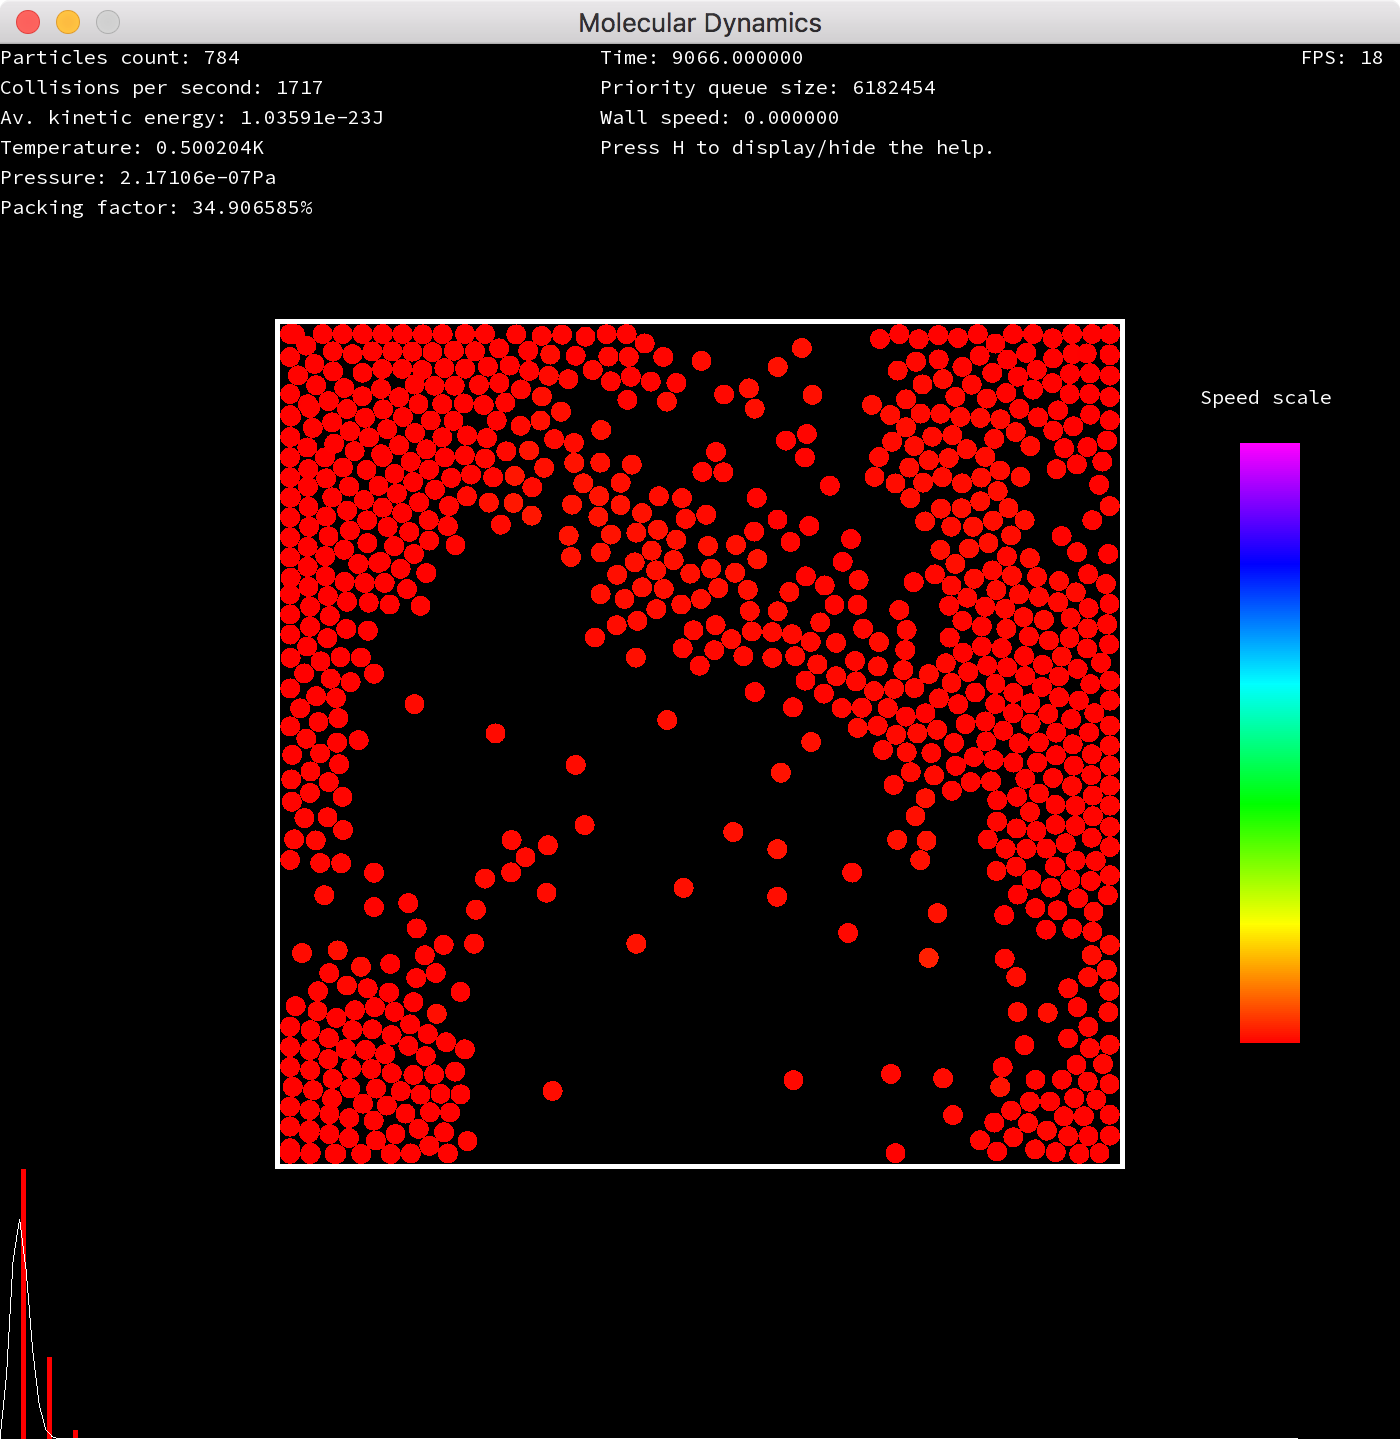
\includegraphics[width=\linewidth]{figures/rotation.png}
    \caption{Mouvement d'ensemble avec les paramètres 10 10 0.6}
  \end{marginfigure}

  \section{Suites et recherches}
  Les différentes possibilités envisageables pour faire évoluer ce programme sont donnés dans le fichier TODO.md. Parmi elles, les plus intéressantes sont :
  \begin{itemize}
    \item Implémenter des collisions multi-particules.

    \item Implémenter l'expérience du démon de Maxwell.

    \item Utiliser un arbre bicolore plutôt qu'une file de priorité pour la gestion des évènements.

    \item Paralléliser les phases de calcul.
  \end{itemize}

  \bibliography{sample-handout}
  \bibliographystyle{plainnat}

\end{document}
